\tocless\chapter{Comptes rendu d'entretiens}
\paragraph{Identification de la personne, exploration du contexte}
	\begin{itemize}
	  \item 1.1. Quel est votre métier ? Quels sont vos rôles et responsabilités ?
	  \begin{description}
	  	\item[Toulouse~:] Responsable intégration / urbanisation. L’objectif du pôle
	  	intégration est d’étudier tous les besoins liés à l’interopérabilité. Ils
	  	sont sollicités dès qu’un chef de projet demande la mise en place d’un
	  	flux, dès qu’une nouvelle application arrive.
	  	\item[Tours~:] Fait partie de l’équipe intégration. Equipe de deux
	  	personnes.
	  	En charge de tous les flux, principalement les flux médicaux. S’occupe un
	  	peu moins des flux administratifs (flux de la logistiques…). Donc
	  	principalement des flux concernant les patients.\\
		L’établissement dispose de plusieurs EAI.
	  	\item[Rouen~:] Fait partie de l’équipe intégration et flux (département RIF),
	  	en binôme avec une collègue, il s’occupe des différents EAI, dont Cloverleaf.
	  	\item[Brest~:] Personnes présentes~: trois personnes utilisant Cloverleaf
	  	par le biais de l’IDE et de EAI Supervision. Profils plutôt techniques.
	  	\item[Metz~:] Travail dans le secteur exploitation, s’occupe principalement
	  	de la gestion des flux.
	  \end{description}
	  
	  \item 1.2. Comment est structuré le service informatique dans votre
	  établissement ? Quels sont les différentes fonctions que l’on y retrouve ? Combien de personnes ?
	  \begin{description}
	  	\item[Toulouse~:] L’interopérabilité : Echanger des données entre
	  	applications métier. Ces applications sont réparties en domaines : soin,
	  	médico-technique, logistique, administratif.\\
		Il y a différents niveaux liés à l’interopérabilité : l’urbanisation,
		l'architecture globale du SI, les normes des données la et mise en œuvre de
		ces normes, l'intégration de nouvelles applications, la surveillance des flux
		(supervision). Bientôt un pôle exploitation va être créé. Ce pôle s’occupera
		de la supervision des flux.
	  	\item[Tours~:] 3 départements : \\
		-	Administratif : admission des patients, logistique, finances, etc.\\
		-	Médicale : Applications médicales\\
		-	Technique : réseau, matériel…
	  	\item[Rouen~:]
	  	\begin{figure}[H]
			\centering
			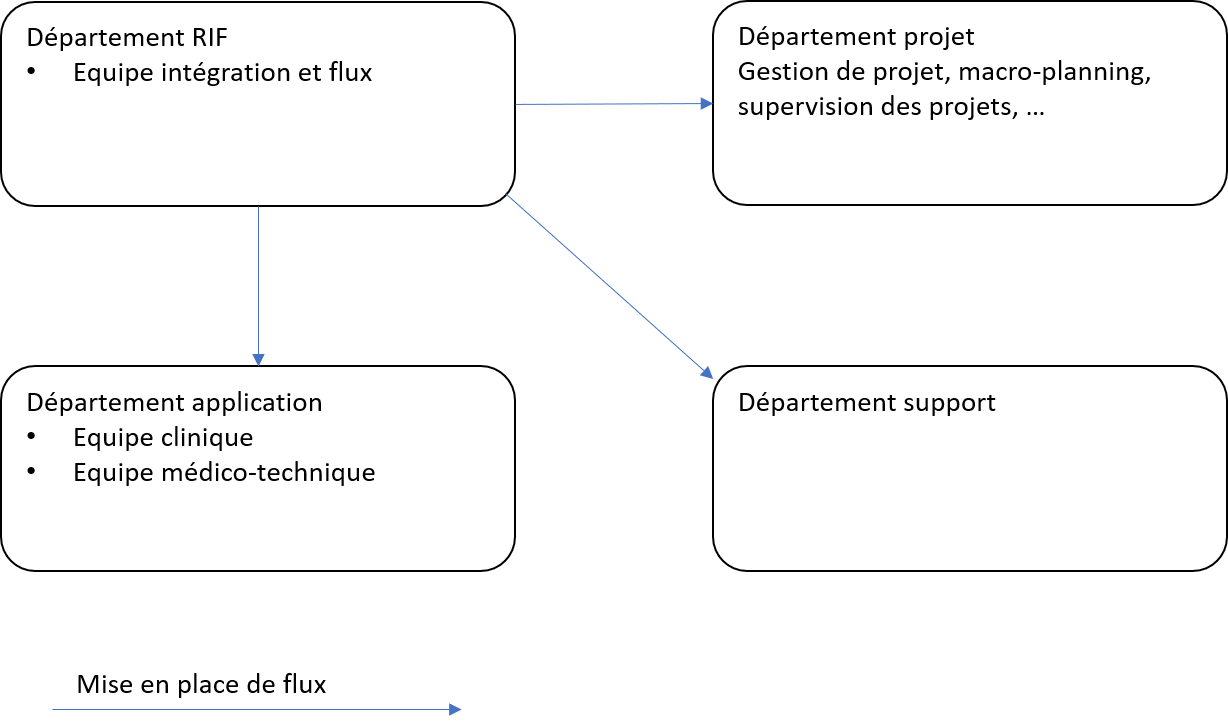
\includegraphics[width=15cm]{../img/annexes/orga_rouen.png}
		\end{figure}
		Le département application est le plus gros demandeur de flux. Les
		départements application et support ont des équipes d’informaticiens qui
		n’ont pas forcément des compétences sur Cloverleaf.
	  	\item[Metz~:]
	  	\begin{figure}[!H]
			\centering
			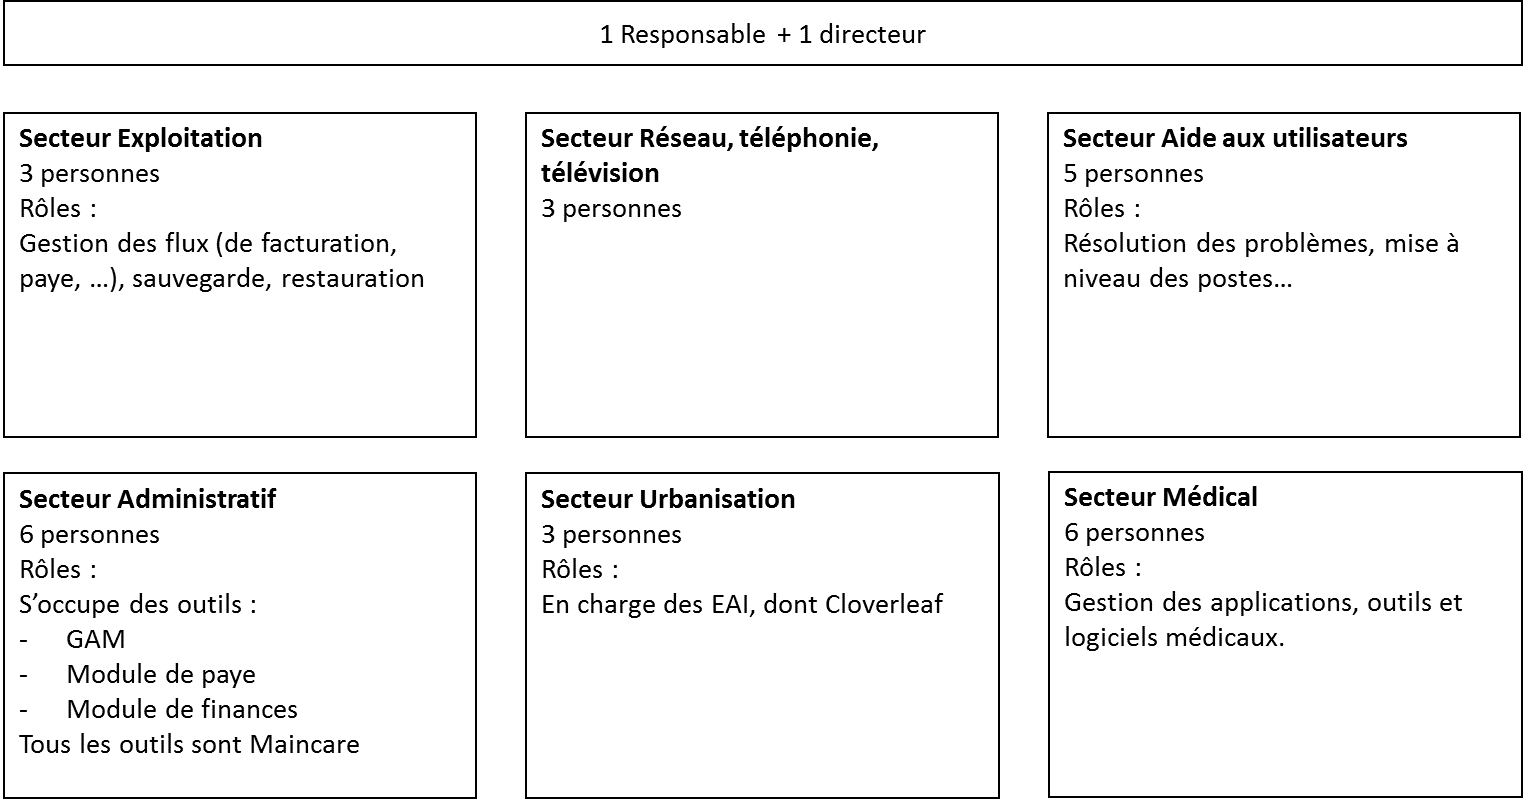
\includegraphics[width=15cm]{../img/annexes/orga_metz.png}
		\end{figure}
	  \end{description}
	  
	  \item 1.3. Quels sont vos liens avec les autres services / les autres
	  fonctions ? (Coopération, liens hiérarchiques, conflits, …)
	  \begin{description}
	  	\item[Tours~:] L’équipe intégration se rattache officiellement au
	  	département médical, mais travail autant avec le département administratif
	  	que médical.
	  	\item[Metz~:] En lien principalement avec le secteur administratif. Peu de
	  	liens avec le secteur réseau, téléphonie, télévision, le secteur médical et
	  	le secteur aide aux utilisateurs. Le secteur médical supervise ses propres
	  	flux (flux issus des applications médicales). Le secteur exploitation
	  	s’occupe essentiellement des flux administratifs. Ne s’occupe pas de
	  	Cloverleaf, c’est le secteur urbanisation qui a la charge du bon
	  	fonctionnement de l’EAI. Le secteur exploitation s’occupe de superviser les
	  	flux.
	  \end{description}
	\end{itemize}
	
	\paragraph{Utilisation et utilisateurs de cloverleaf et problématiques liées à
	la supervision des flux}
	\begin{itemize}
	  \item 2.1. Etes-vous amenés à utiliser l’EAI Cloverleaf :
  	  \begin{description}
	  	\item[Toulouse~:] Démarrage de Cloverleaf en 2006 avec le MIPIH. A l’époque,
	  	le rôle du pôle intégration était seulement de faire de la supervision, le
	  	MIPIH s’occupait de tout. Puis le choix a été fait de monter en compétence
	  	sur l’EAI, notamment sur le développement de flux. L’objectif était de
	  	devenir autonome sur le développement de flux, ce qui est le cas
	  	aujourd’hui.\\
	  	Utilisation des consoles de supervision :\\
	  	Global Monitor :\\
	  	Utilisé pour le niveau 1 (surveillance des flux). Utilisé aussi par les
	  	personnes d’astreinte pour surveiller leurs propres flux. Les personnes
	  	d’astreinte ont des restrictions sur la console.
		Global Monitor est utilisé par les techniciens et ingénieurs de la DSIO et par
		le service intégration.\\
	  	TrackCIS :\\
	  	L’objectif est de le mettre à la disposition des référents techniques.
		Les référents techniques sont des personnes métier qui sont les interlocuteurs
		privilégiés avec la DSIO. Ces personnes (pharmaciens, infirmières, médecins…)
		remontent à la DSIO les problèmes lorsqu'ils surviennent. Quand il s’agit
		d’un problème d’interopérabilité (par exemple un message qui ne transite pas
		correctement d’une application à une autre), la DSIO fait appel au service
		intégration pour le résoudre (si elle n’y arrive pas elle-même).\\
	  	Cette procédure de résolution fait appel à beaucoup d’intermédiaires et
	  	prend beaucoup de temps. L’objectif de TrackCIS est de simplifier la
	  	majorité des cas en donnant au référent métier un outil (TrackCIS) lui
	  	permettant de résoudre lui-même certains problèmes (en rejouant ou en
	  	modifiant les messages).\\
		De plus, la supervision des flux est une perte de temps pour le pôle
		intégration.\\
		Utilisation des alertes Cloverleaf par le pôle intégration et par les équipes
		DSIO.
	  	\item[Tours~:] Principalement par le biais de l’IDE, un petit peut avec
	  	Global Monitor.\\
		TrackCIS n’est pas encore utilisé en production, l’outil n’est pas encore
		paramétré.
	  	\item[Rouen~:] Affichage de Global Monitor sur un écran géant. Visualisation
	  	de l’état des flux et des messages en erreur en temps réel. Cet écran
	  	affiche aussi deux autres consoles de supervision pour leurs autres EAI.\\
		L’IDE est installé sur les postes. Utilisé plus pour le paramétrage des flux,
		le diagnostic et la correction des erreurs.\\
		TrackCIS n’est pas utilisé. Il est en cours de paramétrage. Ils
		réfléchissent encore sur le meilleur moyen de l’utiliser.\\
		Ils font peu de transformations.
	  	\item[Brest~:] Utilisation de Cloverleaf via l’IDE et EAI Supervision.
	  	\item[Metz~:] N’utilise que TrackCIS pour gérer les flux Cloverleaf.
	  \end{description}
	  
	   \item 2.2. Quelle part de votre temps allouez-vous à l’utilisation de
	   Cloverleaf ? (IDE et consoles de supervision) Estimez-vous que ce soit trop ? Pas assez ?
	   \begin{description}
	  	\item[Metz~:] En moyenne 1,5h par jour et par personne. N’estime pas que
	  	c’est une perte de temps.
	  \end{description}
	  
	   \item 2.3. Comment évalueriez-vous votre niveau de maîtrise de Cloverleaf~?
	   \begin{description}
	  	\item[Toulouse~:] L’équipe intégration a pour but d’être autonome sur la
	  	création de flux.
	  	\item[Rouen~:] Bonne maîtrise
	  	\item[Brest~:] Une bonne autonomie par rapport à Cloverleaf, bon niveau de
	  	maitrise :\\
		-	L’établissement a mené des négociations avec Maincare dans le but de
		devenir plus autonome vis-à-vis de Cloverleaf. Ces négociations ont
		abouti à des formations de Maincare, notamment sur la création de flux et de
		\textit{threads}.\\
		-	Le CHU est autonome pour la création de nouveaux flux. Cependant, Maincare
		doit valider chaque nouveau flux mis en place.\\
		-	L’équipe maîtrise la transformation de messages (procédures TCL).\\
		L’équipe SI est très curieuse sur le fonctionnement de l’EAI et très
		désireuse de monter en compétence. Pour eux Cloverleaf n’est pas simplement
		une « boite noir » gérée uniquement par Maincare.
	  	\item[Metz~:] Faible niveau de maitrise de l’EAI, ne maîtrise que la
	  	supervision de certains flux via TrackCIS.
	  \end{description}
	  
	   \item 2.4. Quelles sont les autres personnes qui, dans votre établissement,
	   sont amenées à utiliser Cloverleaf~?
	   	\begin{description}
		  	\item[Toulouse~:] Cloverleaf est trop complexe pour des utilisateurs
		  	métier. D’où l’intérêt d’une console telle que TrackCIS. Cela leur
		  	permettrait de vérifier si un message est bien passé.\\
			Rq : Plus de 30 000 messages passent quotidiennement sur les flux
			identité-mouvement.\\
			A l’heure actuelle, aucun référent métier n’utilise encore TrackCIS, même si des
			tests ont déjà été effectués avec ce type d’utilisateur. Aujourd’hui TrackCIS
			est utilisé par les équipes de la DSIO pour réaliser des tests lors de la
			mise en place de flux au moment de la recette fonctionnelle.
		  	\item[Tours~:] Global Monitor est utilisé par les personnes d’astreinte.
		  	Ce sont des personnes utilisatrices d’applications, pas forcément des
		  	informaticiens.
		  	Ils n’ont qu’un accès restreint aux flux qui les intéresse.\\
			Il ne destine pas TrackCIS à des utilisateurs métier. Il craint qu'il soit
			trop compliqué pour eux de gérer les flux, il y a des risques d’erreur de
			leur part surtout au niveau de la correction des erreurs. Ou alors juste en
			lecture seul (sans possibilité de rejouer ou modifier les messages). «~On ne
			peut pas déléguer la fonction de rejoue à tout le monde~».\\
			L’outil est d’avantage destiné à des informaticiens, ayant une connaissance
			minimum de l’IDE. Ces mêmes informaticiens veulent en effet savoir ce qu’il
			s’est passé en cas de problème.
		  	\item[Rouen~:] Concernant TrackCIS~:\\
			Pas d’utilisateurs actuels. Il est prévu que ce soit des personnes métier
			(EAC) qui utilisent TrackCIS, donc pas des informaticiens (des référents
			informatiques). Par exemple le personnel chargé de l’accueil des patients
			pour bien vérifier que les données qu’ils saisissent diffusent bien dans les
			autres applications. Remarques~: pas de cas d’utilisation très claire pour
			l’instant au niveau de ce type d’utilisateur.\\
			L’utilisation de TrackCIS est ici restreinte au domaine concerné par l’utilisateur
			métier.\\
			Concernant Global Monitor :\\
			Utilisé par tout informaticien travaillant de près ou de loin sur des flux~:
			les informaticiens du département application, du département support et bien
			sur de l’équipe intégration et flux.\\
			L’utilisation de Global Monitor est ici également restreinte au domaine
			concerné par l’utilisateur.\\
			Concernant EAI supervision~:\\
			Utilisé par les informaticiens du département application (et aussi un peu
			par ceux du département support) pour gérer les flux Maincare et
			l’intégration des messages dans les applications de l’éditeur. C’est le département support qui fait le lien
			avec Maincare en cas de problème.
		  	\item[Brest~:] Les mêmes personnes utilisent Cloverleaf via son IDE et EAI
		  	Supervision. Ces personnes sont très compétentes sur l’EAI. La console de
		  	supervision est utilisée pour gagner du temps et visualiser rapidement les
		  	messages en erreur, faire des modifications sur les messages et les
		  	rejouer.
		  	\item[Metz~:] Il a essayé de donner le suivi des flux aux utilisateurs des
		  	applications administratives, mais sans succès. Aucun utilisateur ne
		  	semble vouloir s’occuper de ça, estimant ne pas avoir le temps et que ça
		  	n’est pas leur rôle de le faire. De plus, une pratique est déjà bien
		  	installée : si un envoi de message ne fonctionne pas, l’utilisateur appel
		  	directement le service exploitation.\\
			C’est le seul utilisateur de TrackCIS dans l’établissement.
		  \end{description}
	\end{itemize}
	
	\paragraph{Attentes par rapport aux consoles de supervision}
	Question généraliste (ne s’applique pas à un outil en particulier) :
	\begin{itemize}
	  \item 3.1. Selon vous, quels sont les 3 principaux rôles qu’une console de
	  supervision d’un EAI tel que Cloverleaf ? Autrement dit, quels sont les 3
	  principales problématiques auxquelles de telles plateformes répondent ?
	  \begin{description}
	  	\item[Toulouse~:] Pouvoir visualiser très rapidement les problèmes ; Avoir
	  	une ergonomie simple ; Pouvoir agir pour dépanner (mais ça c’est
	  	facultatif).\\
	  	Le rôle premier d’une console de supervision est de pouvoir
	  	rapidement diagnostiquer un problème. La résolution du problème est une
	  	fonction «~bonus~» de la console.
	  	\item[Tours~:] Vision immédiate (de l’état d’un flux, des messages) et sans
	  	besoin de scroller.\\
		En cas d’anomalie, permet d’analyser le problème.
	  	\item[Rouen~:] Varie en fonction du type d’utilisateur de la console.
	  	\item[Brest~:] Utilisation possible par les personnes en astreinte en
	  	lecture seul, mais cela n’est pas le cas actuellement à Brest
	  	\item[Metz~:] <<~Avoir une vue bien claire avec un message allé et un
	  	message retour. Visualiser les erreurs avec leur contenu et leur
	  	origine.~>>\\
	  	Un affichage épuré, simple, pas surchargé en informations.
	  \end{description}
	\end{itemize}
	
	\paragraph{Questions portant sur les consoles actuelles}
	Pour chaque outil utilisé :
	\begin{itemize}
	  \item 4.1. Trouvez-vous que l’utilisation de cet outil soit simple~?
	  Pourquoi~? Quelles sont les difficultés que vous rencontrez (ergonomie,
	  prise en main…) ?
	  \begin{description}
	  	\item[Toulouse~:] TrackCIS est parfaitement adapté aux référents métier.
	  	Très simple à utiliser, pas besoin de documentation.
	  	\item[Tours~:] TrackCIS : pas encore utilisé en production.\\
		Global Monitor : pas de retours négatifs des utilisateurs concernant
		l’ergonomie et la facilité d’utilisation. Mais Global Monitor est lent,
		l’outil se bloque parfois. Au niveau de l’ergonomie, l’espace de la page ou
		des widget est parfois très mal occupé sur certains écrans (éléments dans un
		coin ou tout en bas et rien autour).
	  	\item[Rouen~:] TrackCIS : simple, épuré et ergonomique\\
		Global Monitor : peu ergonomique (surtout pour la rejoue de messages), plus
		difficile à prendre en main
	  	\item[Brest~:] Pour EAI Supervision~: Outil simple à utiliser, relativement
	  	intuitif, mais la prise en main est difficile. Une vue tableau de bord pratique.
	  	\item[Metz~:] Remarque : il utilise conjointement 2 versions de TrackCIS :
	  	la 1.2.0 pour les flux GAM et GEF (flux internes) et la 1.2.93 pour les
	  	flux externes.\\
	  	Il trouve difficile de jongler entre les 2 TrackCIS et il aimerait un
	  	affichage unique pour gérer les flux internes et les flux externes.\\
		Il souhaiterait arriver sur la liste des flux du jour en arrivant sur la page
		d’accueil de TrackCIS (bouton <<~flux du jour~>> ?). Actuellement, il arrive
		sur les flux correspondant à son dernier filtre. Il est obligé de refiltrer les
		flux à la date d’aujourd’hui chaque jour. Car le suivi des flux <<~se fait au
		jour le jour~>>.
	  \end{description}
	  
	  \item 4.2. Selon vous, quelle est le plus gros atout de cet outil ?
	  \begin{description}
	  	\item[Toulouse~:] TrackCIS permet de donner de l’autonomie aux personnes dont
	  	l’EAI n’est pas le métier. « Les gens sont très contents d’avoir une
	  	certaine autonomie. » TrackCIS permet de renommer les flux (contrairement à
	  	Global Monitor), ce qui est pratique pour les utilisateurs métier qui ne
	  	connaissent pas les codes des informaticiens.
	  	\item[Tours~:] Global Monitor : permet de comprendre ce qu’il s’est passé en
	  	cas d’erreur.
	  	\item[Rouen~:] Pour TrackCIS : \\
		Sa simplicité d’utilisation, ce qui en fait un bon outil pour des utilisateurs
		non informaticiens et non-initiés à Cloverleaf (utilisateurs métier). Peu de
		données affichées, juste le nécessaire pour ce type d’utilisateur. Il
		pense que TrackCIS doit rester à un faible niveau de détail d’information
		pour ne pas perdre ce type d’utilisateur.
	  	\item[Metz~:] La vue d’ensemble sur les flux est très pratique.\\
		Le fait d’avoir le plus de renseignement possible sur un minimum de colonnes.
	  \end{description}
	  
	  \item 4.3. Quelles sont les fonctionnalités que vous êtes amené à utiliser le
	  plus souvent sur cet outil ? Pour quoi ?
	  \begin{description}
	  	\item[Toulouse~:] TrackCIS :\\
		Aller chercher les messages par rapport à un critère donné (le nom d’un patient…).
		Explorer le contenu du message pour voir par exemple pourquoi il n’est pas
		passé.\\
		Global Monitor :\\
		Visualiser l’état des flux, pouvoir voir si les messages transitent bien.
		Voir les problèmes.
	  	\item[Tours~:] Global Monitor~: pour les astreintes, recherche
	  	d’un message à partir de la date et de l’heure, de l’IPP ou de l’IEP principalement.
	  	Permet d’avoir tous les messages concernant un patient par exemple et de
	  	diagnostiquer une erreur généralisée à tous les messages d’un patient.
	  	\item[Rouen~:] Pour Global Monitor~:
		Visualiser les messages en erreur (rouge/vert : avoir quelque chose de très
		visuel à afficher sur un grand écran).\\
		Editer, rejouer des messages.
	  	\item[Brest~:] Pour EAI Supervision~:\\
	  	- Consultation des messages\\
		- Rejoue de messages\\
		- Alertes\\
		- Pouvoir comparer un message entre l’entrée et la sortie du flux
	  	\item[Metz~:] Ne s’intéresse qu’aux anomalies. Si un message est en erreur,
	  	il va le rejouer après l’avoir édité pour corriger l’erreur, s’il le peut.
	  	S’il ne peut pas (ce qui représente « 97\% des cas »), il appelle la
	  	personne concernée du service administratif pour comprendre l’origine de l’erreur
	  	et la corriger. Par exemple il peut s’agir d’une erreur de saisi de l’un
	  	des utilisateurs de l’application de départ. La correction d’une erreur
	  	peut durer de 48h à 1 mois.\\
		Le fait de savoir que tel message est parti de tel endroit, à telle heure, et
		est arrivé correctement à tel autre endroit.
	  \end{description}
	  
	  \item 4.4. Selon vous, quelle est la plus grosse faiblesse de l’outil ?
	  \begin{description}
	  	\item[Tours~:] Global Monitor a un temps de réponse très long, et se bloque
	  	parfois.\\
	  	Attend de TrackCIS un temps de réponse plus court.\\
	  	La recherche de message à partir de l’IPP ou de l’IEP est difficile.
	  	\item[Rouen~:] Pour Global Monitor :\\
		La gestion des erreurs n’est pas très pratique. Pas de widget dédié aux
		erreurs. Il est difficile de voire rapidement, en un coup d’œil s’il y a eu des
		erreurs et lesquelles. De plus, il n’est pas possible de trouver la cause de
		l’erreur directement dans la console, il faut forcément entrer dans
		l’\textit{error database}.\\
		Pour TrackCIS~:\\
		Les colonnes sont difficiles à paramétrer. Le système d’adresse de champ n’est
		pas intuitif, il faut bien connaitre la nature des flux et des messages, bien
		connaitre les standards. Or l’application est destinée à des utilisateurs qui
		ne connaissent pas forcément tout ça. Il verrait bien la possibilité de
		sélectionner dans une liste déroulante le champ que l’on veut voire en colonne.
		Par exemple~: pour le format XML, utiliser un parseur XML qui donnerait les
		balises disponibles dans une liste.\\
		Dans ces conditions, il serait intéressant que l’utilisateur métier puisse
		lui-même choisir ses colonnes.
	  	\item[Brest~:] Pour EAI Supervision~:\\
	  	Un peu lent.
	  	\item[Metz~:] TrackCIS rend transparent le fonctionnement de Cloverleaf et
	  	notamment la nature des flux. L’utilisateur (qui n’a jamais toucher à
	  	l’EAI) ne connait pas l’architecture d’un flux (d’où viennent les messages,
	  	par où ils passent, les transformations qu’ils subissent, si c’est crypté,
	  	où ils vont et s’il y a des retours).\\
		L’affichage d’un grand nombre de message est trop lent, par exemple quand il
		souhaite afficher 100 messages par pages ce qui induit une perte de temps.
	  \end{description}
	  
	  \item 4.5. Citez au moins 3 fonctionnalités qui vous semble manquer dans cet
	  outil ?
	  \begin{description}
	  	\item[Toulouse~:] TrackCIS :\\
		Ajouter des libellés à certains éléments de contenu des messages. Par exemple
		associer le libellé «~admission~» au code «~a04~». Ces libellés et ces codes
		sont propre à un format de message donné. Il faudrait permettre à
		l’administrateur d’un TrackCIS de créer des tables de correspondance entre code et
		libellé au niveau d’un flux donné ou d’un format donné.\\
		Au démarrage de TrackCIS on arrive sur la liste des messages qui prend du
		temps à s’afficher car une requête est faite sur toute la base. Quand il y a beaucoup
		de messages, ça peut prendre plusieurs minutes. Il faudrait que les messages
		ne se chargent pas directement au démarrage de TrackCIS.\\
		BONUS~: pouvoir créer des profils d’utilisateur.\\
		Pouvoir gérer les formats fixes comme le format FRL.\\
		Global Monitor~:\\
		Avoir des statistiques sur les flux dans un but de reporting auprès de la
		direction.\\
		Donner accès à la documentation de niveau 1 sur les flux ainsi qu’aux
		consignes de résolution de problèmes.\\
		Pouvoir ranger les flux dans l’ordre
		que l’on veux.
	  	\item[Tours~:] Pouvoir consulter les scripts \textit{xlate}. Ces
	  	informations sont parfois utiles pour les informaticiens qui utilisent l’outil. Les scripts
	  	ne sont pas toujours bien répertoriés dans l’établissement et sont souvent
	  	difficiles à retrouver quand on en a besoin.
	  	\item[Rouen~:] TrackCIS : ne trouve pas de fonctionnalités à ajouter
	  	\item[Brest~:] - Pouvoir remonter à la source de l’utilisateur. Notamment
	  	pour corriger les erreurs humaines (erreurs de saisie). Les erreurs de
	  	saisie sur des données médicales sont impossibles à corriger par l’équipe
	  	SI. Il faudrait pouvoir envoyer un mail à l’utilisateur pour qu’il corrige
	  	son erreur.\\
		- Pouvoir gérer l’intégration des messages dans les applications. En général,
		les éditeurs des applications métier donnent accès aux CH aux BDD. «~Avoir une
		partie dynamique qui irait chercher des informations dans la BDD des
		applications~».
	  	\item[Metz~:] Il faudrait une documentation rapide et schématique de chaque
	  	flux. Documentation en ligne accessible depuis TrackCIS ou intégrée à
	  	TrackCIS.\\
		Pour les flux externes, les messages en KO n’apparaissent pas dans la liste des
		messages en erreur. Il perd donc beaucoup de temps à scroller et à parcourir
		toutes les pages pour les trouver, surtout quand il y a beaucoup de
		messages.\\
		Dans la liste des messages, voir le nombre de message en ARL+ sur le nombre
		de messages total.\\
		Enfin, il souhaiterait voir afficher, en plus du numéro de la page où il se
		trouve, le nombre de messages correspondant. Par exemple : Page 2 (messages 101
		à 200 / 1234), Page 3 (messages 201 à 300 / 1234), etc.
	  \end{description}
	  
	  \item 4.6. Si l’outil pouvait afficher des statistiques sur les flux (comme
	  par exemple le nombre de messages en erreur heure par heure, …), quelles
	  données seraient les plus pertinentes à afficher selon vous~? (En proposer au
	  moins 3 en précisant le mode d’affichage (graphique, histogramme, tableau,
	  …))
	  \begin{description}
	  	\item[Toulouse~:] Nombre de messages, nombre d’erreurs par flux, par site.
	  	Pouvoir éditer un rapport mensuel et l’exporter pour l’envoyer à la
	  	direction. Quelque chose de simple et de « jolie » qui permet de rendre
	  	compte de tout ce qui transite par l’EAI et que tout se passe bien.\\
		Il peut être intéressant de voir le temps de transfert des messages dans l’EAI.
		Ça permettrait de rendre compte et de comprendre le retard d’un message.
	  	\item[Tours~:] Volumétrie / jour / \textit{process} ou \textit{thread}.
	  	Nombre de message et volume de données (octets).
	  	\item[Rouen~:] Temp d’intégration d’un message. Temps de transfert et temps
	  	de traitement d’un message de l’application A à l’application B.
	  	Visualisation de ce temps par message et en moyenne. C’est une donnée qui pourrait intéresser
	  	l’utilisateur métier. Exemple~: un tableau des messages avec une colonne
	  	dédiée au temps, la moyenne affichée quelque part (moyenne au jour, semaine,
	  	mois …)\\
	  	Remarques :\\
		Au niveau des utilisateurs métier, les services d’urgence travaillent toujours
		en flux tendu. Ils ont donc besoin d’une vision en temps réel. A l’inverse,
		les mêmes types d’utilisateurs dans d’autres services n’ont besoin que
		d’une vision plus globale.\\
		L’\textit{error database} est difficile à comprendre, il est difficile de
		comprendre la cause d’une erreur.
	  	\item[Brest~:] - Garder des informations sur le nombre de messages tombés en
	  	erreur et le nombre de messages rejoués sur une période donnée.\\
		- L’objectif et de se faire une idée du temps passé à corriger les erreurs, de
		visualiser le volume de messages en erreur (pour un jour donné par exemple) et
		le nombre de ces erreurs qui ont pu être corrigées. Permet de valoriser
		l’activité des administrateurs de Cloverleaf.
	  	\item[Metz~:] Il serait intéressé par des statistiques, mais sur un autre
	  	onglet, pas de stats dans la liste des messages (risquerait d’encombrer
	  	l’affichage et de diminuer la clarté de l’outil).\\
		Pourcentage de messages tombés en erreur sur un pas de temps donné (jour,
		semaine ou mois). Nombre de fichiers envoyés.\\
		Vitesse moyenne du transfert des messages dans l’EAI.\\
		Le tout par flux et avec la possibilité de choisir son pas de temps (jour,
		semaine, mois).
	  \end{description}
	  
	  \item 4.6 bis. Quelles données statistiques (présentent dans le
	  \textit{status} dans l’IDE) vous sont les plus utiles au quotidien~?
	  \begin{description}
	  	\item[Toulouse~:] La première chose qu’elle regarde le matin c’est la date
	  	de dernière écriture d’un message. Permet de voir directement si les
	  	messages passent ou pas (car en principe, les messages circulent en flux
	  	continu).
	  	\item[Tours~:] D’abord les messages en entrée et en sortie puis le nombre de
	  	messages en attente et enfin les dates de dernière écriture de message en
	  	entrée et en sortie. L’objectif est de vérifier que le \textit{thread}
	  	fonctionne, qu’aucun message n’est bloqué.
	  	\item[Rouen~:] Son processus de diagnostic et de correction d’une erreur
	  	(message tombé en erreur)~:\\
		1)	Dans le clic droit \textit{status}, il regarde la date et heure de dernière
		écriture d’un message (s’il voit que des données ont été écrites récemment,
		c’est qu’il n’y a pas eu de blocage)\\
		2)	Va vérifier les \textit{logs} du \textit{process} \\
		3)	Va vérifier le ou les messages concernés dans les SMAT
	  \end{description}
	  
	  \item 4.7. Que pourrait vous apporter de telles statistiques ? (Plus
	  d’efficacité dans la gestion des messages, meilleure vision globale…) En quoi
	  cela changerait vos pratiques ?
	  \begin{description}
	  	\item[Toulouse~:] Reporting sur le bon fonctionnement de l’IDE auprès de la
	  	direction. Permet la certification du SI. Le reporting est un gage de
	  	qualité, la preuve que tout marche bien.\\
		Les statistiques n’intéresseraient pas les référents métier directement. En
		revanche, la direction pourra être amenée à publier ces stats en internes de
		façon à ce que les référents puissent les consulter.
	  	\item[Tours~:] L’évolution de la volumétrie peut être révélatrice de
	  	problèmes.
	  	\item[Metz~:] Cependant, il ne voit pas encore bien en quoi ces stats
	  	pourraient améliorer sa gestion des flux.\\
		Selon lui, les stats permettent de faire un suivi, mais pas d’aider à corriger
		les erreurs.
	  \end{description}
	\end{itemize}